\documentclass{article}
\usepackage{mystyle}
\usepackage{Sweave}
\begin{document}
\Sconcordance{concordance:documento.tex:documento.Rnw:%
1 2 1 1 0 13 1}
\Sconcordance{concordance:documento.tex:./tex/lab2.Rnw:ofs 17:%
1}
\Sconcordance{concordance:documento.tex:documento.Rnw:ofs 18:%
18 1 1}
\Sconcordance{concordance:documento.tex:./tex/lab3.Rnw:ofs 20:%
1 55 1}
\Sconcordance{concordance:documento.tex:documento.Rnw:ofs 76:%
21 1 1}
\Sconcordance{concordance:documento.tex:./tex/lab4.Rnw:ofs 78:%
1}
\Sconcordance{concordance:documento.tex:documento.Rnw:ofs 79:%
24 1 1}


\title{Optimizació Numérica}
\author{Manuel Sarmiento Navarro}
\maketitle

% \section{Introducción}
% \SweaveInput{tex/intro.Rnw}

% \section{Laboratorio 1}
% \SweaveInput{tex/lab1.Rnw}
% 
\section{Laboratorio 2}
Laboratorio 2

\section{Laboratorio 3}
\begin{enumerate}
  \item Demostrar que $\min_{v}\{||x-v||:w^{T}v + b = 0\} = |w^{T}x + b|$
  
  \item Demostrar que el modelo \emph{duro} de \emph{máquinas de soporte vectorial}:
  \begin{gather*}
  \argmax\limits_{(w,b):||w||=1} \min_{i\in[m]}|w^{T}x_{i}+b| \\
  \text{s. a. } y_{i}(w^{T}x_{i}+b) > 0 \quad \forall \quad i \in [m] \\
  \end{gather*}
  se puede reescribir como 
  $$
  \argmax\limits_{(w,b):||w||=1} \min_{i\in[m]}y_{i}(w^{T}x_{i}+b)
  $$
  
  \item Probar que este problema se puede resolver con 
  \begin{gather*}
  (w_{0},b_{0}) = \argmax\limits_{(w,b)} ||w||^2 \\
  \text{s. a. } y_{i}(w^{T}x_{i}+b) \geq 1 \quad \forall \quad i \in [m] \\
  \hat{w} = \frac{w_{0}}{||w_{0}||}, \quad \hat{b} = \frac{b_{0}}{||w_{0}||}
  \end{gather*}
  
  \item Reescribir el problema anterior como un programa cuadrático de la forma
  \begin{gather*}
  \frac{1}{2}x^TPx + q^Tx \\
  \text{s. a. } Gx \leq h \\
  Ax = b
  \end{gather*}
  
  \item Escribir la función \verb|hard_svm()| en Python que resuelva el problema anterior usandlo \verb|cvxopt|
  \begin{lstlisting}[language=Python]
  def hard_svm(X, y):
    '''
    (X,y): Datos de entrenamiento [X.shape=(m,p), y.shape=(m,)]
    X,y matrices de numpy
    (w,b):  Hiperplano [w.shape=(p,), b.shape=(1,)]
    '''
    P = matrix(np.concatenate((np.concatenate((np.identity(X.shape[1], float), np.zeros((X.shape[1],1),float)), axis=1), np.zeros((1,(X.shape[1]+1)),float)), axis=0), tc='d')
    q = matrix(np.zeros((X.shape[1]+1,1),float), tc='d')
    y.shape = (X.shape[0],1)
    X = np.concatenate((X, np.ones((X.shape[0],1))), axis=1)
    G = -y * X
    G = matrix(G, tc='d')
    h = matrix(-np.ones(X.shape[0]), tc='d')

    sol = solvers.qp(P,q,G,h)
    print(sol['x'])
    w = np.array(sol['x'])
    w, b = w[0:-1,:], w[-1,:]

    return w, b
  \end{lstlisting}
  
  \item Al graficar la el hiperespacio que resulta de aplicar la función \verb|hard_svm()| a los puntos  \verb|(X,y) = datos(200)| se obtiene:
  \begin{figure}[H]
    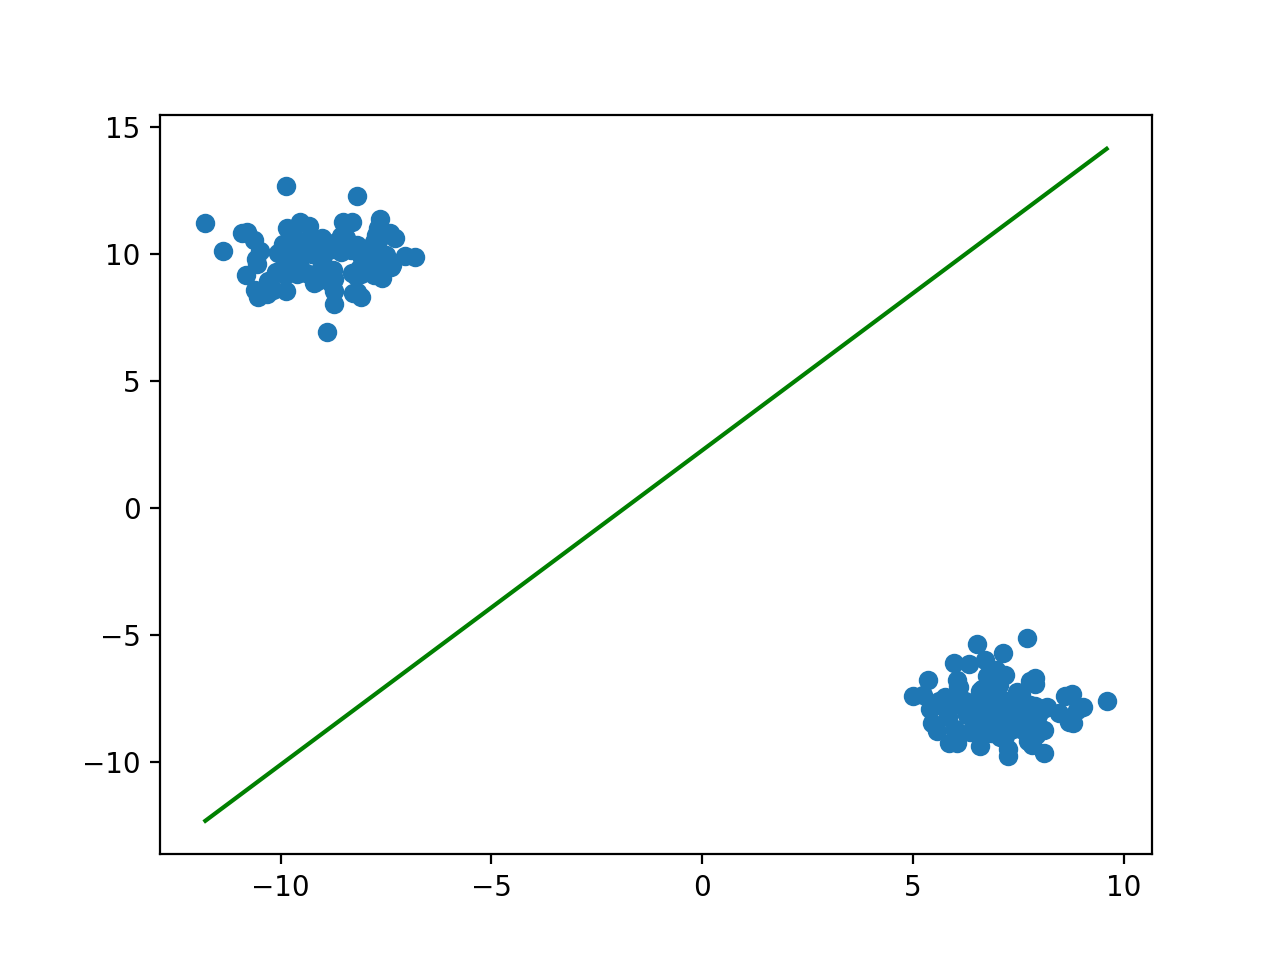
\includegraphics{img/hsvm200.png}
  \end{figure}
\end{enumerate}

\section{Laboratorio 4}
Laboratorio 4

\end{document}
